\documentclass[useAMS, usenatbib, a4paper]{mnras}
\pdfsuppresswarningpagegroup=1
% \RequirePackage{amsmath}
% \documentclass[times]{aastex63}
% \usepackage{natbib}
\usepackage[spanish,es-minimal,english]{babel}
\usepackage[utf8]{inputenc}
\usepackage{graphicx}
%\usepackage{microtype}
\usepackage{xcolor}
\usepackage{fixltx2e}
\usepackage{hyperref}
\usepackage{savesym}
\savesymbol{tablenum}
\usepackage{siunitx}
\restoresymbol{SIX}{tablenum}
\usepackage{newtxtext}
\usepackage[varg,varvw,smallerops]{newtxmath}
\usepackage{xfrac} % for the \sfrac macro
\usepackage{booktabs}
\usepackage{array}   % for \newcolumntype macro
\newcolumntype{L}{>{$}l<{$}} % math-mode version of lrc column types
\newcolumntype{R}{>{$}r<{$}} 
\newcolumntype{C}{>{$}c<{$}}
\hypersetup{colorlinks=True, linkcolor=blue!50!black, citecolor=black,
  urlcolor=blue!50!black}

\usepackage{etoolbox}
\robustify\bfseries
\robustify\itshape
\usepackage{enumerate}

\bibliographystyle{mnras}

\sisetup{
  % explicit""+" is useful for velocities
  retain-explicit-plus = true,
  % prefer 10^6 over 1 x 10^6
  retain-unity-mantissa = false,
  % Use x +/- e instead of x(e)  
  separate-uncertainty = true,
  % Make sure to pick up bold font when used in section heading for instance
  detect-weight = true,
}
\DeclareSIUnit\msun{\text{M\ensuremath{_\odot}}}
\DeclareSIUnit\lsun{\text{L\ensuremath{_\odot}}}

% A better \ion command that works in more circumstances
\newcommand\ION[2]{#1\,\scalebox{0.9}[0.8]{\uppercase{#2}}}
\newcounter{ionstage}
\renewcommand{\ion}[2]{\setcounter{ionstage}{#2}% 
  \ensuremath{\mathrm{#1\,\scriptstyle\Roman{ionstage}}}}
\newcommand\hii{\ion{H}{2}}

% Stars in Orion, e.g., \th1C, \th2A
\def\th#1#2{\ensuremath{\theta^{#1}\,\text{Ori~#2}}}
% Wavenumbers
\newcommand\wn{\ensuremath{\tilde{\nu}}}

% Chemical formulae
\newcommand*\chem[1]{\ensuremath{\mathrm{#1}}}
% Atomic term symbols
\newcommand\Config[1]{\ensuremath{\mathrm{#1}}}
\newcommand\Term[3]{\ensuremath{\mathrm{#1\ ^{#2}#3}}}
\newcommand\Level[4]{\ensuremath{\mathrm{#1\ ^{#2}#3_{#4}}}}

% Emission lines
\newcommand\ha{\ensuremath{\text{H}\alpha}}
\newcommand\hb{\ensuremath{\text{H}\beta}}
\newcommand\lya{\ensuremath{\text{Ly}\alpha}}
\newcommand\lyb{\ensuremath{\text{Ly}\beta}}

\newcommand\Raman{\ensuremath{_{\text{Raman}}}}
\newcommand\scat{\ensuremath{_{\text{scat}}}}
\newcommand\FUV{\ensuremath{_{\text{FUV}}}}
\newcommand\wing{\ensuremath{_{\text{wing}}}}
\newcommand\lamcont{\ensuremath{_{\lambda, \text{cont}}}}
\newcommand\observed{\ensuremath{^{\text{obs}}}}
\newcommand\intrinsic{\ensuremath{^{\text{int}}}}
  


\title[Neutral gas in 30 Dor]
{Neutral gas from $b$ to $z$:
  Optical diagnostics of photodissociation regions in 30 Doradus
}

\author[Henney]{
  Mabel Valerdi\textsuperscript{1}
  William J. Henney\textsuperscript{2}\thanks{w.henney@irya.unam.mx}
  and C. R. O'Dell\textsuperscript{3}
  \\
  \textsuperscript{1}\foreignlanguage{spanish}{%
    Instituto Nacional de Astrofísica, Óptica y Electrónica,
    Tonanzintla, Puebla, México}\\
  \textsuperscript{2}\foreignlanguage{spanish}{%
    Instituto de Radioastronomía y
    Astrofísica, Universidad Nacional Autónoma de México, Apartado
    Postal 3-72, 58090 Morelia, Michaoacán, Mexico}\\
  \textsuperscript{3}%
  University of Vanderbilt, Tennessee, United States
}

% These dates will be filled out by the publisher
\date{Accepted XXX. Received YYY; in original form ZZZ}

% Enter the current year, for the copyright statements etc.
\pubyear{2021}


\begin{document}
\label{firstpage}
\pagerange{\pageref{firstpage}--\pageref{lastpage}}
\maketitle



\begin{abstract}
  A detailed study of the neutral interface between ionized and
  molecular gas at the surface of 4 molecular clouds in the
  mini-starburst region 30~Doradus in the Large Magellanic Cloud.
\end{abstract}
\begin{keywords}
  Atomic physics
  -- ISM: individual objects (Orion Nebula)
  -- Photodissociation regions
  -- Radiative transfer
\end{keywords}
%\facilities{VLT:Yepun (MUSE); OANSPM:2.1m (Mezcal); Keck (HIRES)}
%\object{M42}
\section{Introduction}
\label{sec:introduction}

Rayleigh scattering describes the absorption of a photon, followed by the immediate re-emission of a photon of the same wavelength. On the other hand, Raman scattering describes the absorption of a photon, followed by the immediate re-emission of a photon at different wavelength (at a much lower frequency.). Both processes begin with a radiation-induced transition of an electron to a virtual bound state (non-eigenstate). 


\citet{Chevance:2016c} used Herschel spectroscopy to study the ``density, radiation field and ISM structure'' in 30 Doradus on scales larger than 12 arcsec. 


\section{30Dor Data}

We use MUSE observations from \citet{Castro:2018a}

\section{Raman scatterd - wings}

\section{CO}

\section{Stars}


{\bf Wavelength bands used for Raman wing extraction}

\begin{table}
\centering
\caption{Wavelength bands}
\label{tab:bands}
\begin{tabular}{lccc}
\hline
 & Band & $\lambda_{min}$\AA  & $\lambda_{max}$\AA \\
\hline
Blue wing & B133 & 6414.85 & 6445.45 \\
          & B080 & 6469.25 & 6496.45 \\
          & B054 & 6499.85 & 6517.70 \\
          & B053 & 6518.55 & 6540.65 \\
Red wing  & R040 & 6594.20 & 6611.20 \\
          & R058 & 6612.05 & 6628.20 \\
          & R087 & 6638.40 & 6660.50 \\
          & R136 & 6688.55 & 6708.95 \\
\hline
\end{tabular}
\end{table}


\begin{figure}
\centering
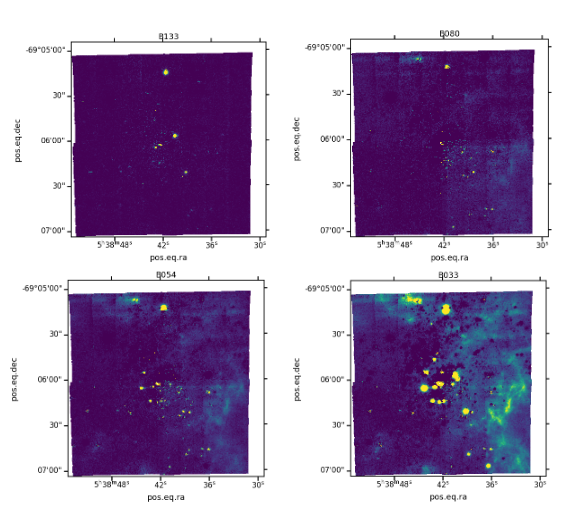
\includegraphics[width=\columnwidth]{Figures/B_band.png}
\caption{Blue Band}
\label{fig:BB}
\end{figure}

\begin{figure}
\centering
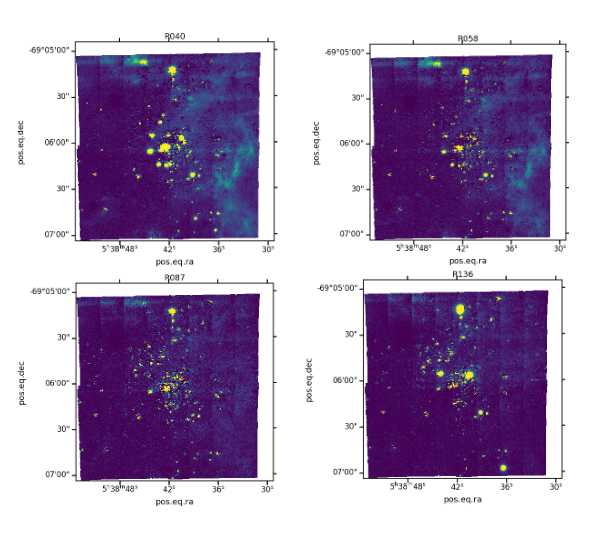
\includegraphics[width=\columnwidth]{Figures/R_band.png}
\caption{Red Band}
\label{fig:RB}
\end{figure}

\begin{figure}
\centering
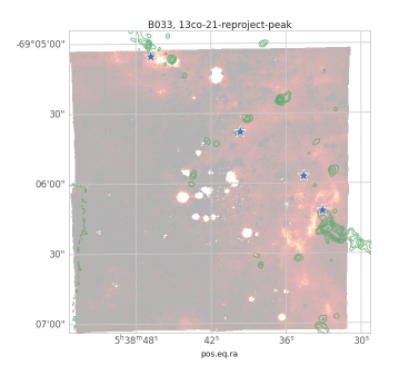
\includegraphics[width=\columnwidth]{Figures/stars.png}
\caption{Stars}
\label{fig:stars}
\end{figure}

\begin{figure}
\centering
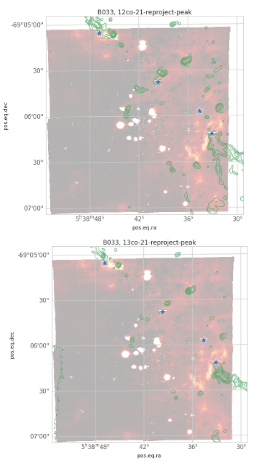
\includegraphics[width=\columnwidth]{Figures/CO.png}
\caption{CO}
\label{fig:CO}
\end{figure}









\newpage

\section*{Acknowledgements}

\bibliography{mabel-tarantula-refs}




% Don't change these lines
\bsp	% typesetting comment
\label{lastpage}

\end{document}
%%% Local Variables:
%%% mode: latex
%%% TeX-master: t
%%% End:
